% !TeX root = ../thesis.tex

\chapter{系统评估}

本章重点介绍在 FPGA 上对系统的构建和评估,实验的目标主要分为以下几个方面:

\begin{itemize}
    \item 验证硬件实现的正确性;
    \item 验证软件实现的正确性;
    \item 验证软硬件协同设计的用户态中断的性能优势;
    \item 分析测试结果与硬件行为间的联系。
\end{itemize}

\section{实验环境}

\begin{figure}
    \centering
    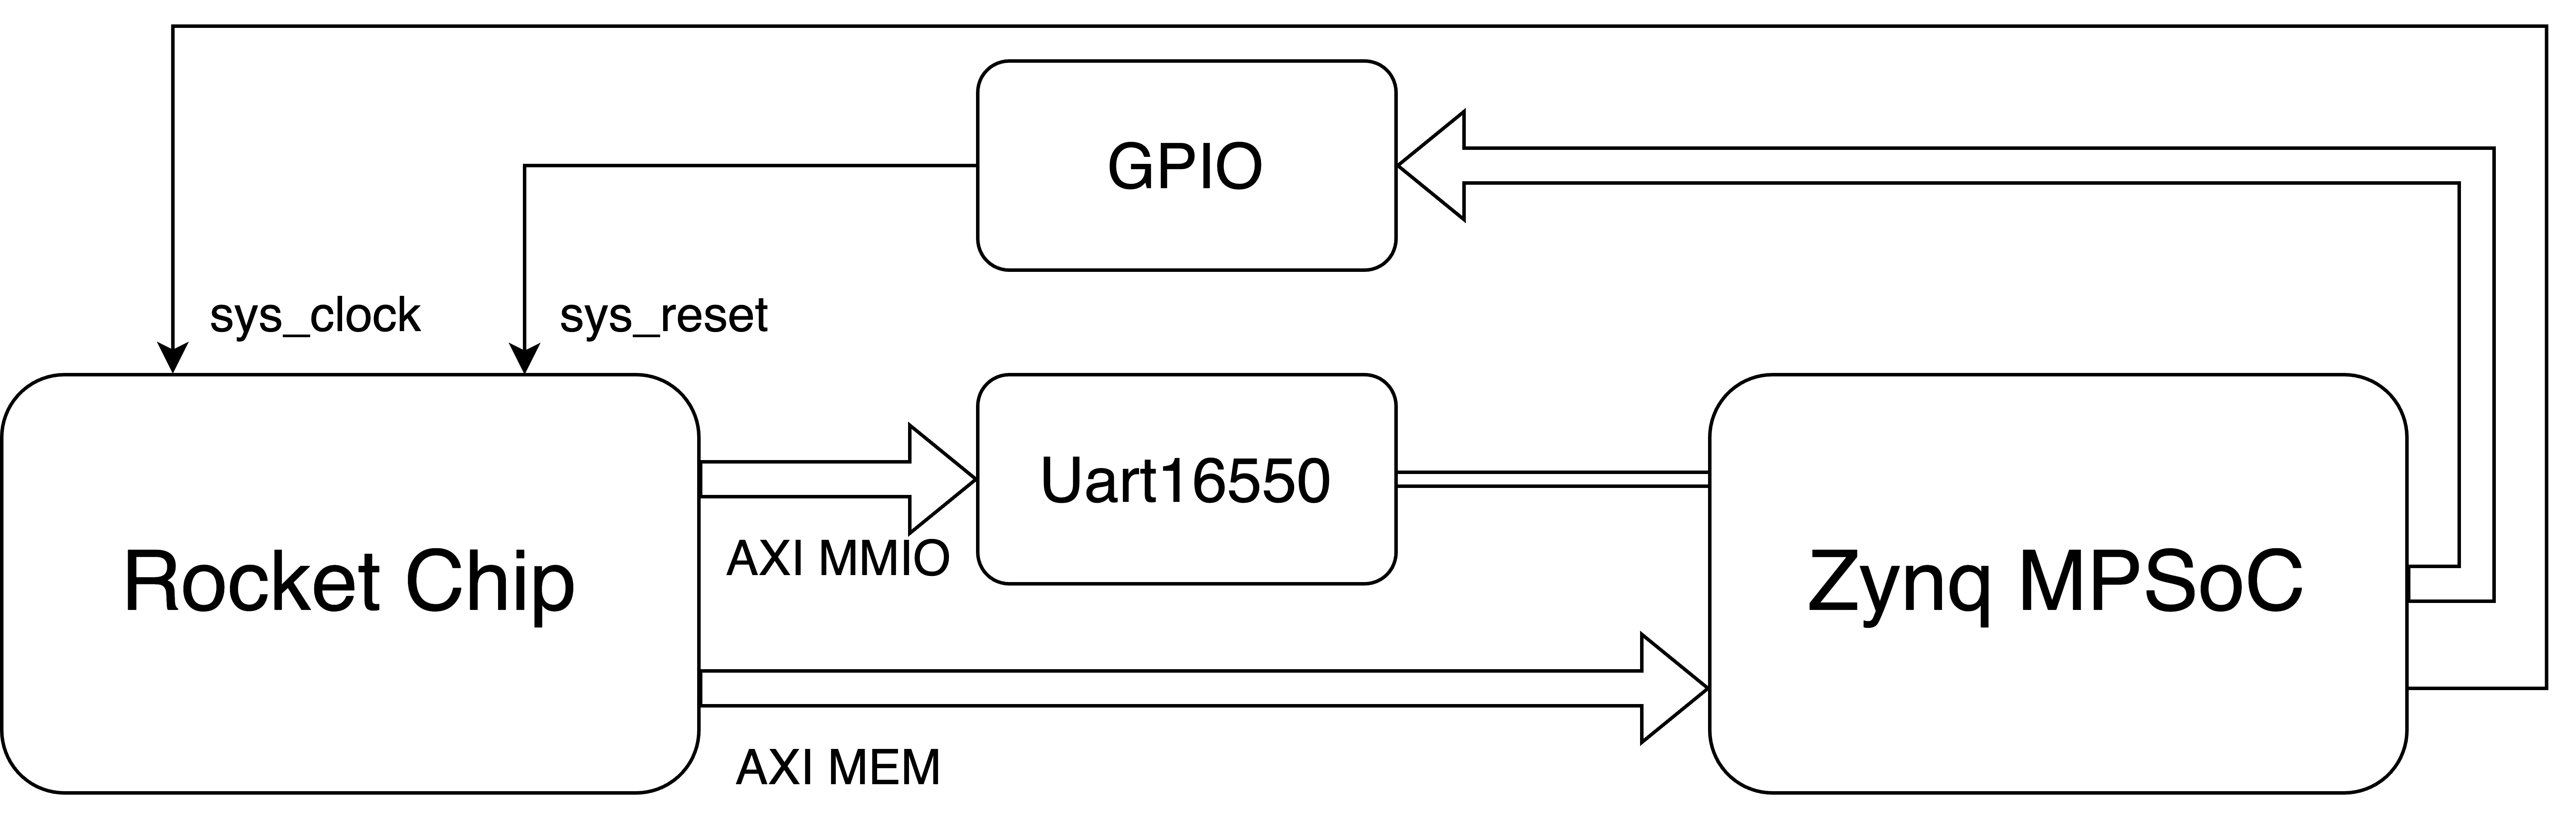
\includegraphics[width=0.8\linewidth]{figures/soc.png}
    \caption{SoC 整体架构}
    \label{fig:soc}
\end{figure}

本文实验主要在 Zynq UltraScale+ MPSoC ZCU102 开发板上开展。ZCU102 分为两个部分,分别为处理器子系统(PS) 和 可编程逻辑(PL) 。PS 提供一款四核 ARM® Cortex®-A53、双核 Cortex-R5F 实时处理器,可以直接对开发板上的资源进行控制;PL 端可以通过 DDR4 组件访问内存资源。

首先,应用 Xilinx 提供的 petalinux SDK 构建在 PS 上运行的 Linux 系统,并挂载 SD 卡作为系统的存储外设。如图 \ref{fig:soc} 所示,引入 AXI GPIO IP 核并在 PS 的设备树给出相关信息,GPIO 的出端口连接到 Rocket Chip 内部,可以在 PS 上操作 /sys/class/gpio/* 来写入这个端口对 Rocket Chip 进行复位。

利用 Rocket Chip 支持的自定义端口和自定义配置参数构建顶层模块。自定义配置包括加入第三章最后一节介绍的 UIPI 协处理器,设置 BootROM 的地址和加载内容。Rocket Chip 顶层模块需要对外暴露两个 AXI master 接口,MEM 端口访问位于 PS 端的 DDR 控制器,MMIO 端口访问 PL 上引入的 Uart16550 IP 核。关于两个端口的地址映射,需要将 Rocket Chip 配置的映射和 Block Design 构建时指定的地址映射相对应。

进一步地,定义系统的顶层模块对 Rocket Chip 顶层模块和 Block Design 模块进一步封装,该模块会对 AXI 接口的位宽进行处理,此外,由于 Rocket Chip 默认看到的内存起始地址为 0x80000000 ,而 Block Deisgn 中 DDR 控制器访问端口的地址映射起始地址为 0 ,需要在模块中对地址高位进行截断。

为了与 Rocket Chip 上运行的系统软件进行交互,引入 Uart16550 IP 核,虽然 Rocket Chip 能够自动生成与内部配置有关的设备树信息,但缺少 PL 额外引入的设备的设备信息,需要手动加入 Uart16550 的设备树节点。

\begin{figure}
    \centering
    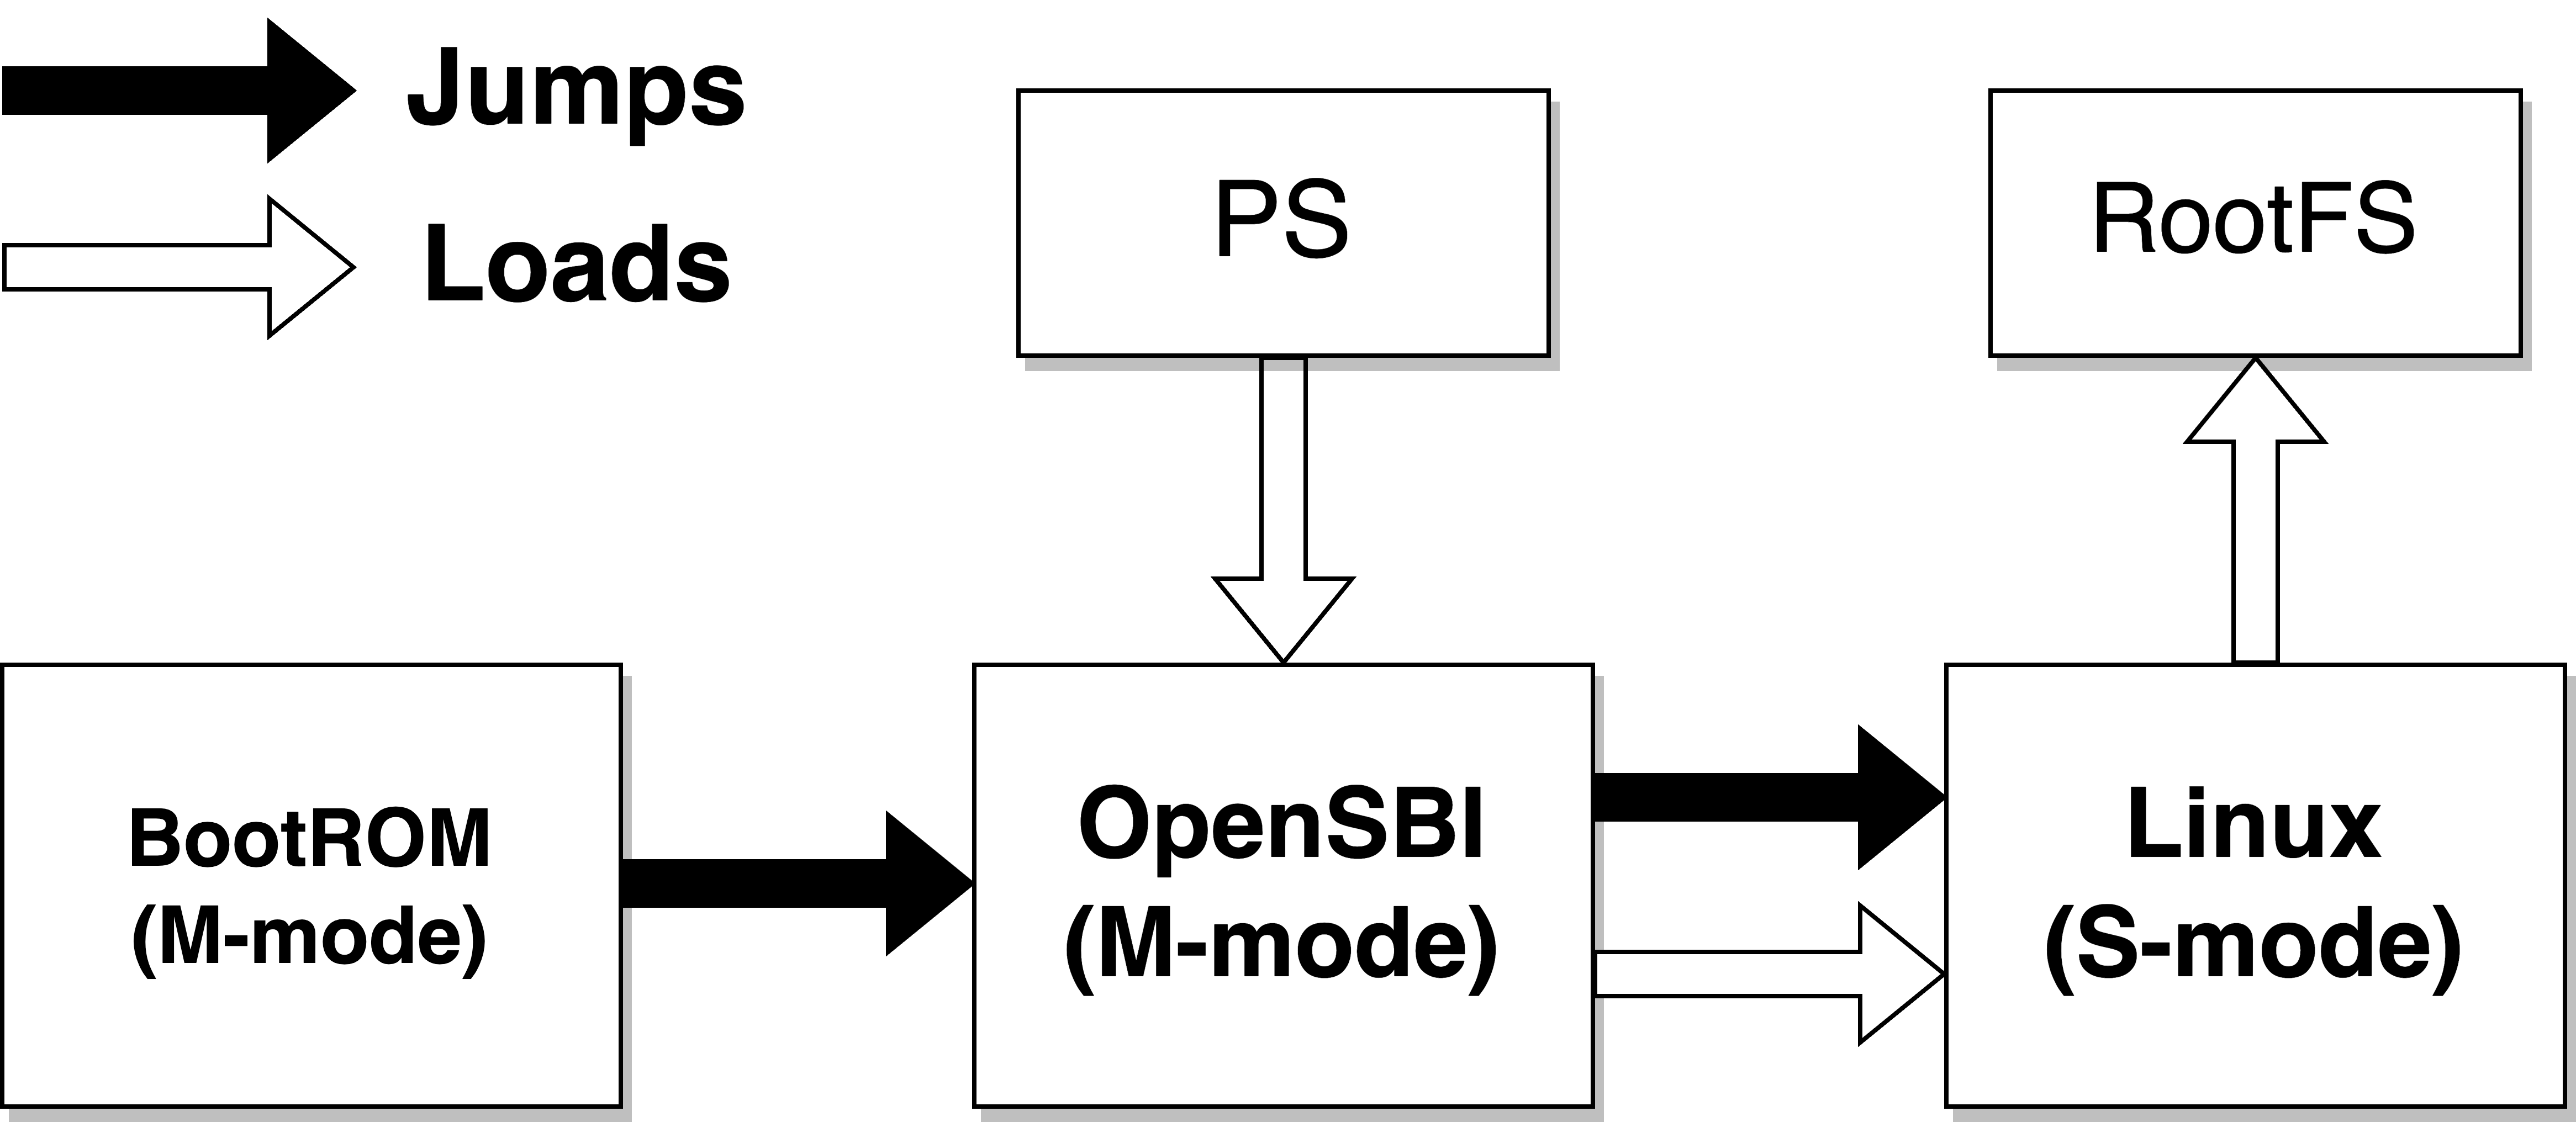
\includegraphics[width=0.8\linewidth]{figures/boot.png}
    \caption{系统软件启动流程}
    \label{fig:boot}
\end{figure}

系统软件的启动流程如图 \ref{fig:boot} 所示。BootROM 为 Rocket Chip 内置的启动代码,在构建时会提前写入到模块中,跳转地址默认为内存的起始地址。

OpenSBI (RISC-V Open Source Supervisor Binary Interface) 是 RISC-V 架构下的 Bootloader,支持通用 SBI 接口,支持 dynamic、jump、payload 三种启动方式。本文的实验采用 payload 启动方式,OpenSBI 镜像会根据 Linux 镜像和设备树的文件位置一起构建。OpenSBI 会在运行时将 Linux 镜像加载到目标地址,并将设备树放在指定的地址。跳转到 Linux 镜像前,OpenSBI 会将核号、设备树地址等信息传递给 Linux 用于 Linux 进一步的初始化。

Buildroot 是一个构建嵌入式 Linux 系统的框架。本文的实验使用 Buildroot 构建根文件系统,并在 Linux 的编译选项中指定文件系统镜像的位置,让 Linux 镜像与文件系统镜像一起构建,并将该文件系统作为 initramfs 。此外,为了让 Linux 在启动时可以打印日志,需要在设备树中添加启动参数指定 earlycons 。

如前文所述,PS 可以对 Rocket Chip 进行复位,在复位前,需要把构建好的 OpenSBI 镜像拷贝到内存中,这部分内存以 reserved-memory 的形式挂载到 PS 的 /dev/mem 文件上,PS 可以直接对该文件进行 mmap 操作完成镜像的写入。

Linux 启动后,可以在主机上连接开发板的串口并看到输出:

\section{功能测试}

\subsection{Verilator 仿真测试}

\subsection{软件接口测试}

根据图 \ref{fig:uintr2} 中 RISC-V 用户态中断的工作流程,可以实现一个简单的进程间通信应用。

\begin{lstlisting}[style=CStyle]
    volatile unsigned int uintr_received; // volatile 避免编译优化
    unsigned int uintr_fd;

    uint64_t uintr_handler(struct __uintr_frame *ui_frame, uint64_t irqs) {
        uintr_received = 1; // 设置标志位
        return 0;
    }

    void *sender_thread(void *arg) {
        int uipi_index;
        // 注册发送方状态表项
        uipi_index = uintr_register_sender(uintr_fd);
        // 发送用户态中断
        uipi_send(uipi_index);
        return NULL;
    }

    int main() {
        pthread_t pt;
        int ret;
        // 注册接收方中断处理函数
        if (uintr_register_receiver(uintr_handler))
            exit(EXIT_FAILURE);
        // 注册文件描述符
        ret = uintr_create_fd(1);
        if (ret < 0) exit(EXIT_FAILURE);
        uintr_fd = ret;
        // 创建发送方
        if (pthread_create(&pt, NULL, &sender_thread, NULL))
            exit(EXIT_FAILURE);
        // 忙等待标志位
        while (!uintr_received);
        pthread_join(pt, NULL);
        close(uintr_fd);
        // 正常退出
        exit(EXIT_SUCCESS);
    }
\end{lstlisting}

接收方注册中断处理函数,注册文件描述符,创建发送方进程,并忙等待标志位;发送方进程注册后发送一个中断便直接退出;接收方收到中断并陷入中断处理函数后设置标志位,回到正常流程发现标志位已被设置,继续执行直到退出。

\section{性能测试}

\section{测试结果分析}